
\chapter{Introduction to Complexity Theory}


Chapter~\ref{chap:languagesautomaten} studies the decidability of
languages, and which machinery is needed to do that. Once it is clear
that a language $L$ is decidable, the game changes: we know there
exists algorithms for deciding whether a string belongs to $L$, and we
are now interested in the {\em cost} of a particular algorithm, the
inherent cost of the problem, and even the {\em best} algorithm. All
this must be made more precise.

Cost is always expressed in units of a particular type. We have two
natural types for the cost of an algorithm: its time and its space
usage. In this chapter, time is dominant. In daily life, we measure
time in (multiples of) seconds. That time unit is difficult to
formalize. Also, we would prefer not to depend on the technology at
hand, because technology changes. We are lucky: there exists a
universal technology: the Turing machine. Time means nothing to a TM,
but we have the notion of an elementary operation that covers the
execution of TM: one application of $\delta$. That unit is used as
{\em time unit}. We will at some point criticize this model, but it
stands very firm. To be more precise on the model: the TM has one
tape that is unbounded in both directions; the read/write head can
move to the left, to the right, or stay on the same cell at each
transition.

To get insight in the performance of an algorithm, someone could
prepare for you a tabel with for a number of input strings $s$ the
time $time_A(s)$ the algorithm $A$ uses for deciding about $s$.
It is difficult to do that for enough relevant strings, and it is
difficult to interpret correctly such a tabel. We must find a better
way to play this game. It is reasonable to expect, and this is true
for most reasonable/interesting algorithms, that (roughly) {\em the
longer $s$, the higher $time_A(s)$}. It is therefore reasonable to
express the performance of $A$ as a function $time_A$ that maps the
length $n$ of an input string on one of the following quantities:

\begin{verse}
- the minimal time $A$ uses to decide a  string $s$ with $|s| = n$

- the average time $A$ uses to decide a  string $s$ with $|s| = n$

- the maximal time $A$ uses to decide a  string $s$ with $|s| = n$
\end{verse}

We use the latter: it s known as the {\em worst case time complexity}
of $A$. A formal definition follows soon.

In this chapter the following topics are treated:

\begin{verse}
- time complexity of a Turing machine
\\
- the class \P and its robustness
\\
- certificate and verifier
\\
- two definitions of the class \NP
\\
- polynomial reduction and $\N$P-completeness
\\
- examples of $\NP$-complete problems: SAT, HAMPATH ...
\\
- the time hierarchy
\\
- co-\NP and $\overline{\NP}$
\\
- en introduction to space complexity
complexity
\end{verse}




\section{Time complexity of algorithms}
 
\grijs{\begin{definitie} Time complexity of an algorithm\\
{ The {\bf time complexity} of an algorithm $A$ is a function
  $time_A(n):\N\rightarrow \N$ that maps an input size $n$ to the
  maximally needed steps performed by $A$ on any input string of size
  $n$:

~~~~~~~~~~~~~~~~~~~~$time_A(n) = max(\{time_A(s)|~|s| = n\})$ }

$time_A(s)$ is the number of steps $A$ performs to decide $s$.
\end{definitie}}

The definition shows that $time_A(n)$ is a {\bf worst case}
measure. It is quite possible that the algorithm needs much less time
than $time_A(n)$ for most strings with length $n$ and that only a few
exceptional strings $s$ with that length really need $time_A(n)$.

In general, complexity theory emphasizes the performance of an
algorithm on large input. Since the exact time needed for one step in
a TM is not clearly defined, the time complexity of an algorithm is
relevant only up to a constant\footnote{And don't forget the linear
  speedup theorem!}. Therefore, the following definition comes in
handy:

\grijs{\begin{definitie} The big $O$-notation (pronounce as {\em big
      oh)}\\
{ let $f,g$ be functions with signature $\N$ to $\R^+$. We say
$f(n)$ is $O(g(n))$ (or $f$ is $O(g)$, and we write also
  $f(n)=O(g(n))$) if
\[\exists c\in \R_0^+,\; \exists N\in \N,\;
\forall n\in \N: \; n\geq N \Rightarrow f(n)\leq c.g(n)\]

We also say: f is of order g, and $f$ is asymptotically dominated by
$g$.  }
\end{definitie}}

 

Note: it is possible that for particular $f$ and $g$, both $f$ is
$O(g)$ and $g$ is $O(f)$ are true, but that does not mean they are
equal.

\begin{vb}{
The function mapping $n$ on $3n^2+4n +3$ is $O(n^2)$, because
\[ 3 n^2+4n +3 \leq 4 n^2,\;\; \forall n\geq 5 \;\;(c=4,\;\;N=5).\]
On the other hand, $n^2$ is also $O(3n^2+4n +3)$ because
\[ n^2 \leq 3 n^2+4n+3,\;\; \forall n\geq 0 \;\; (c=1,\;\; N=0). \]
}
\end{vb}

{\bf A selfie:} prove that a positive polynomial with degree $k$ is
$O(n^{k+i})$ if $i \geq 0$, but not if $i < 0$; prove that the
relation {\em dominates asymptotically} is transitive; provide two
functions $f$ and $g$ so that $f$ is not $O(g)$ and (at the same time)
$g$ is not $O(f)$.



\grijs{\begin{definitie} Asymptotic equivalence of functions.\\
{ Two functions $f,g:\N\rightarrow \R^+$ are asymptotically equivalent
  if
\[ f\mbox{ is }O(g)\mbox{ and } g \mbox{ is } O(f) \]
We denote this by $f$ is $\theta(g)$ (or $g$ is $\theta(f)$).
}
\end{definitie}}



{\bf A selfie:} {\em asymptotically equivalent} is an equivalence
relation; two positive polynomials are asymptotically equivalent if
and only if they have the same degree.



The $O$-concept provides a means to compare algorithms. Suppose two
algorithms $A$ and $B$ solve the same problem. Let $time_A(n)$ and
$time_B(n)$ their complexity functions. $A$ is better (for large
input) than $B$ if 

\begin{enumerate}
\item $time_A(n)$ is $O(time_B(n))$, and
\item $time_B(n)$ is not $O(time_A(n))$
\end{enumerate}

So, if we have an algorithm $A$ with linear complexity
(i.e. $time_A(n)$ is $O(n)$) and an algorithm $B$ with quadratics
complexity function ($time_B(n)$ is $O(n^2)$), we consider $A$ the
better algorithm.  One should however not conclude that algorithm $A$
is always to be preferred over $B$: the constant factor $c$ in the
definition of big oh could be very large for $A$ and small for $B$,
meaning that if $n$ remains small, $B$ could be more efficient.

To get a bit more insight in the notion of complexity, it pays off to
know the asymptotic behavior of some functions. The sequence below
gives the asymptotic behavior of some important functions: a function
$f(n)$ is to the left of $g(n)$ if $f(n)$ is $O(g(n))$ (and not the
other way around).
\[ \log_2 n \;\; n\;\; (n\log_2 n)\;\;  n^2\;\; \cdots\;\; n^k\;\;
\cdots\;\; \;\;2^n \;\; n!  \]




\grijs{\begin{definitie}\label{TtimeTM} Let $T$ be a function with
signature$ \N \rightarrow \R^+$. We say that a Turing machine $M$ runs
in time $T$ if $M$ stops on every input $s$ after at most $T(|s|)$
steps.
\end{definitie}}

We also say {\em $M$ is a $T$-time Turing machine}. The algorithm
implemented by $M$ is of course $O(T)$, but the converse is not
true. (Why not?)



\grijs{\begin{definitie} A polynomial algorithm\\
{ An algorithm is {\bf polynomial} if its time complexity is $O(n^k)$
for some $k\in \N$.}
\end{definitie}}

 



\grijs{\begin{definitie} An exponential algorithm\\
{ An algorithm is {\bf exponential} if its time complexity is
$\theta(c^n)$ for some real number $c>1$.}
\end{definitie}}


A quick comparison shows that exponential algorithms are eventually
less efficient than polynomial algorithms. Suppose that a particular
problem can be solved by algorithm $A$ with $time_A(n)=n^5$, and also
by $B$ with $time_B(n)=2^n$. On a machine that can execute 10 million
instructions each second, $A$ solves a problem of size $n=60$ in
less than 2 minutes, while $B$ needs more than 3500 years. We say {\em
$B$ scales badly}.

It feels like it is in our interest to have polynomial algorithms for
particular problems. That is however not always possible, and even it
is, the degree of the polynomial might be too high for practical
purposes. Other methods will need to be employed in that case: these
methods are not part of this course.



\paragraph{What if we use other types of machines?} Many other
computing formalisms are Turing-complete, so it feels a bit arbitrary
to build complexity theory starting from TMs. We will later see why it
works anyway. Another attack on TMs would be that one could express
the cost of an algorithm in terms of the number of elementary
operations needed, as for instance the comparison of swapping of two
array elements. One can read sentences like {\em quicksort is
$O(n^2)$}, but the $n$ is the number of items to sort, not the size of
the input. The $n^2$ is a (worst case) measure for the number of
comparisons, and indeed, for quicksort that is $O(n^2)$. But one
comparison takes many steps on a TM, and moreover depends on the size
of the representation of the numbers to compare. On top of that, {\em
sorting} is not a decision problem ...


\paragraph{To decide or to compute?}

A decider behaves like a function whose range has only two values:
accept and reject. On the other hand, we can interpret the contents
of the tape at the end of a decision process as the result of a
computation. If we look at it that way, the TM $M_f$ implements a
function $f$ with range $\Sigma^*$. You can construct a TM $M_{fbit}$
with input a tuple $\langle s,i,b \rangle$ - the TM accepts if the
$i$-th bit of $f(s)$ equals $b$: $M_{fbit}$ uses $M_f$ as a {\em
subroutine}\footnote{Please make the construction more explicit}. This
shows a strong link between deciding and computing. It also works the
other way around: if you get $M_{fbit}$, you can build $M_f$ (even if
$M_{fbit}$ does not have $M_f$ inside) ... well, almost ... What is
missing?


\begin{sloppypar}
\paragraph{Non-deterministic time complexity classes}
We later need a complexity measure for non-deterministic Turing
machines (NDTM). The non-deterministic analogue of
Definition~\ref{TtimeTM} is
\end{sloppypar}

\grijs{\begin{definitie}\label{TtimeNDTM} Let $T$ be a function with
signature $\N \rightarrow \R^+$. We say that a non-deterministic
Turing machine $M$ runs in time $T$ if $M$ stops on every input $s$
after at most $T(|s|)$ steps for each choice of the transition.
\end{definitie}}


\section{Time complexity of languages or decision problems}


Now we know about the time complexity of algorithms, we could try to
determine the {\em best} algorithm for a given language $L$. That
would give a characterization of the inherent difficulty of the
problem. That approach fails in most cases. Still, there is a way to
get some understanding of the difficulty of a problem.

\subsection{Time complexity classes}



\grijs{\begin{definitie} DTIME(T)\\
{ DTIME(T) is the set of languages that can be decided by a
  (deterministic) $c.T$-time Turing machine, with $c > 0$.}
\end{definitie}}


$NDTIME(T)$ is similar but for a decision by a $c.T$-time NDTM.

{\bf A selfie:}
\begin{verse}
if $f = O(g)$, then $DTIME(f) \subseteq DTIME(g)$

$DTIME(T) \subseteq NDTIME(T)$
\end{verse}

The next definition captures the class of languages that can be
decided by a polynomial Turing machine:

\grijs{\begin{definitie} \P = $\cup_{k\geq 1} DTIME(n^k)$
\end{definitie}}

\paragraph{Examples of languages in \P}
\begin{itemize}
\item 
$Sum = \{\langle a,b,c \rangle| a,b,c \in \N \wedge a+b=c\}$
\item 
$Sorted = \{[a_1,a_2,...,a_n]| a_i \in \N \wedge (a_i \leq a_{i+1})\}$
\item 
$Connected = \{\langle G \rangle|G~is~a~connected~graph\}$
\end{itemize}

\paragraph{The definition of \P is robust.} 
We previously committed to expressing the time complexity function on
a Turing machine with one read/write two-sided tape, and with the
possibility for the head to not move. What happens to $\P$ if we use
another machine ? The answer is ...{\em nothing} on condition we keep
it reasonable: more than one tape, one-side tape ... it does not
matter. We can even use random-access machines, n-dimensional tapes
... Each of those variant TMs can be simulated by the type of TMs we
committed to, with only a polynomial overhead. It because tricky when
one would allow one memory cell to contain an arbitrarily large
number, or count some arithmetic operations on such numbers as unit
cost. For instance, it would be weird (but scientifically valid) to
define the time cost of the $n^{th}$ step during a T execution as
$2^{-n}$\footnote{This machine is known as a Zeno-machine.}: each
algorithm takes at most one time unit ... and we can fold the
complexity theory books.


\paragraph{Outside of \P ...} 
Some problems cannot be solved in polynomial time. The class of
languages that need at most exponential time contains such languages:

\grijs{\begin{definitie} \EXP = $\cup_{k\geq 1} DTIME(2^{n^k})$
\end{definitie}}

It should be clear that $\P \subseteq \EXP$. The inclusion is even strict: see Section~\ref{timeshierarchie}.
%
The complement of \EXP is is not empty: Presburger arithmetic provides
an example.

\paragraph{How about the encoding?}
It is time to worry about the encoding of a problem, or of a language.
A decision problem is usually formulated without direct reference to
its possible encoding. For instance: we can talk about the language of
even numbers, or the problem to decide whether a number is odd or
even. Once the encoding is fixed, we can construct an algorithm, and
then perhaps determine its complexity.

For numbers, we have (at least) two natural encodings: we can use a
unary alphabet, or a binary one. In the unary one, the number $2048$
has representation length 2048, in binary one, it has length 12. Let
us imagine a $TM_u$ and a $TM_b$ for either encoding. The best
possible $TM_u$ needs to count (modulo 2) the number of characters in
$s$, so it is $O(|s|)$. The best $TM_b$ needs to skip all characters
until it finds the last one, and then takes the decision: it is
$O(|s|)$ as well. But in terms of the size of the number represented
by $s$, the binary representation is superior: for deciding about
$2048$, $TM_b$ needs a little more than $log_2(2048)$ steps, while
$TM_u$ needs about 2048. On the one hand, both algorithms have linear
complexity, on the other hand, the unary encoding needs exponential
more time for deciding the same number.

A second example makes it worse: consider a naive algorithm to decide
whether a number $n$ is prime. It has a loop of the form

\begin{algorithmic}
    \State{i := 2}
    \While {$i \leq n$}
         \If{i divides n}
         \State{REJECT;}
         \State{i += 2;}
         \EndIf
    \EndWhile
    \State{ACCEPT}
\end{algorithmic}

In both encodings, the loop is executed $n$ times, but in terms of the
size of the encoding, that is exponentially more with the binary
representation than with the unary one. In one case we could think
that the algorithm is polynomial, in the other case that it is
exponential.

Clearly, we need to agree on the encoding in order to talk
unambiguously about the complexity of a problem and an algorithm. Here
is rule number one: for numbers do not use the unary encoding. You may
use binary, ternary or decimal ...: that makes no real difference
since all these representations can be transformed into each other at
only a polynomial cost. For other objects, we might have to find an
ad-hoc agreement, or sometimes, it is clear that some encodings are
bad. For graphs, we should use the adjacency matrix. Think up some
unreasonable representation for graphs, and explain why it is.


\subsection{The complexity of multiplication: an excursion}

For convenience, we use the decimal representation of numbers.
We can consider the multiplication of two numbers in the range $0..9$
as elementary. How many elementary multiplications do we need to
multiply two numbers? For simplicity, we consider numbers of the same
length (add zeros if needed):$a= a_na_{n-1}...a_1$, and
$b = b_nb_{n-1}...b_1$. We want to compute $a \times b$. At school, we
learned to do this with $n^2$ elementary multiplications,and some
additions. People have thought for a long time that it could no be
done with essentially less: the grat A. Kolmogorov even has put this
forward as a conjecture he strongly believed in. A. Karatsuba showed
that it is possible anyway.

Again for simplicity, assume that $n$ is even and equal to $2m$. Then
one can write $a$ and $b$ as
%
$a = A_{2}10^m + A_1$ en $b = B_{2}10^m + B_1$.
%
Then 

$~~~~~~~~~~a \times b = (A_{2}\times B_{2})10^{2m} + (A_{2}\times B_1 + A_1\times B_{2})10^m + A_1\times B_1 $ \\
in which you can see 4 multiplications.

A. Karatsuba noticed that the coefficient of $10^m$ can be computed in
a different way:

$~~~~~~~~~~(A_{2}\times B_1 + A_1\times B_{2}) = (A_{2} + A_1) \times (B_{2} +
B_1) - (A_{2}\times B_{2}) - (A_1\times B_1)$. \\
In the last two multiplications give the coefficients of $10^{2m}$ and
$10^0$. By remembering the result of the last two multiplications, and
reusing it, one now gets $a \times b$ in only 3 multiplications.
By applying this principle recursively (divide and conquer) the number
of elementary multiplications is $O(n^{log_2(3)})$. In the mean time,
algorithms with an even lower complexity have been discovered.

What did we learn from this excursion? Sometimes, intuition tells us
that there is only one possible way to compute a result, and later we
learn we were wrong: there is another (better) way, perhaps many other
ways.

\subsection{Certificates and verifiers}

The concepts of certificate and verifier are introduced here
independent of their use in complexity: you must be able to understand
and interpret their definitions (and properties) without referring to
complexity.


\grijs{
\begin{definitie}\label{verifiercertificate}
A {\bf verifier} for a language $L$ is a deterministic TM $V$
such that 

~~~~~~~~~~~~~~~~~~~~~~
$\forall s \in \Sigma^* : (s \in L \leftrightarrow \exists c \in \Sigma^*: V(\langle s,c \rangle) = accept)$


$c$ is named the {\bf certificate} for $s$
\end{definitie}
}

Some examples:
\begin{itemize}
\item 
let $L$ be the set of composite numbers; there exists of course a TM
$M$ that decides that language: a typical algorithm would try to find
a divisor for a given number. However, if a number $n \in L$ than
there exists a divisor $d$, and we could give the numbers $n$ and $d$
to a TM $V$ that verifies thatr $d$ is indeed a divisor of $n$: $V$
has less work to do than $M$, and according to the definition, it is a
verifier for $L$, while the given divisor $d$ is the certificate. Note
that it impossible to fool or mislead the verifier: you cannot make it
accept a prime as a composite

\item 
let $L$ be the language of tuples of the form $\langle G,a,b \rangle$
in which $G$ is a graph, and $a$ and $b$ are vertices connected by a
path in $G$; once more, there exists a TM $M$ that decides exactly
this language, by just trying to construct a path; a verifier $V$ can
be easier: a possible certificate is a path between $a$ and $b$; $V$
merely needs to check that this certificate is really a path in $G$,
starting with $a$ and ending with $b$; verifying something is a path
is easier than constructing it: $V$ needs less work than $M$; try to
fool $V$ ... it is impossible

\item
let $L$ be the set of TMs $M$ for which $L_M$ is not empty; we showed
earlier that this language is not decidable; still, for every TM $M$
with $L_M \neq \emptyset$, there is a certificate that it is in $L$,
namely any $c \in L_M$; the verifier just runs $M$ on $c$

\end{itemize}

The first two examples give the intuition that the job of a verifier
for $L$ is easier than the job of a decider for $L$. The last example
makes it blatantly clear: the language does not need to be decidable
in order to have a verifier/certificate.

Confused? Think about it, reread Definition~\ref{verifiercertificate}.

It might have escaped your attention:
Definition~\ref{verifiercertificate} does not mention strings that do
{\bf not} belong to the language. You get to know something about such
strings by juxtaposition. You get: for $s \notin L$, every $c$ is {\bf
not} a certificate.

Think about this: the definition of verifier/certificate says nothing
about strings {\bf not} in the language.

The intuition holds up: a verifier must work less than a decider. Some
questions remain:
\begin{itemize}
\item 
does every language have a verifier and a certificate for each string
in the language?
\item
can a string have more than one certificate?
\item 
how difficult is it to construct (by an algorithm) a certificate? is
that always possible?
\end{itemize}

The second question above has {\em yes} as answer for each of the
three examples: every divisor is a certificate for a composite number;
every path is a certificate for the fact that $a$ and $b$ are
connected; every $s \in L_M$ is a certificate.

As for the last question: for the first two examples, the certificate
can be generated by an algorithm (although nobody knows whether it can
be done in polynomial time in the first example); in the third
example, no algorithm can generate a certificate for each
string. Think about this: it might be a bit more subtle than you think
at first.

An additional question can be asked about the length of the certificate:
\begin{itemize}
\item 
is there a relation between the length of $s \in L$ and the length of
its certificate, and the complexity (or decidability) class of $L$?
\end{itemize}
Consider all three examples and comment on that question.


Suppose there is a function $f$ so that for a verifier $V$ and
certificate $c$ for $s$, the length of $s$ is bounded above by
$f(|s|)$, or:
%
$|c| \leq f(|s|)$. Now we can generate a certificate as follows for
any $s \in L$ as follows:

\begin{algorithmic}
    \ForAll {$(i \leq f(|s|) \wedge (c \in \Sigma^i)$}
         \If {$V(\langle s,c \rangle)$ accepts}
         \State{ACCEPT}
         \EndIf
    \EndFor
    \State{REJECT}
\end{algorithmic}

This deterministic algorithm\footnote{Is it an algorithm or can you
turn it into one?} tries all potential certificate candidates. Can we
say something about its complexity?


\begin{itemize}
\item
in the worst case, the for-loop is executed $O(2^{f(|s|)})$ (we assume
the alphabet has two elements)
\item 
if $M$ is a $g$-time machine, the cost of the body of the for-loop is
$O(g(|s|+|c|))$, or $O(g(|s|+f(|s|)))$
\item
this results in an overall complexity $O(g(n+f(n))\times 2^{f(n)})$
where $n$ is the size of the input
\end{itemize}

If $f$ and $g$ are at least linear, the complexity of this algorithm
is exponential or worse, even if $g$ is not. You might feel like
arguing that for some problems there is a less naive way to generate
certificates (think about the connected vertices), and you are right
... but there are quite a lot of problems for which science has not
achieved that. We will see more about this later.

The algorithm above {\em guesses systematically} for a
certificate. One can model that with a non-deterministic procedure,
e.g. by a Prolog predicate. It can also be modelled with a
non-deterministic Turing machine {\em NDTM$_V$} with just two
transitions at each stage. On input $s$, {\em NDTM$_V$} writes in its
first $f(|s|)$ steps non-deterministically a string from
$\Sigma^{f(|s|)}$ on the tape. It then calls the deterministic
verifier $V$. If one of the branches accepts, $s$ is accepted.
Figure~\ref{nondetverifier} illustrates this: the length of the
certificate is 2.


\begin{figure}[h]
\begin{center}
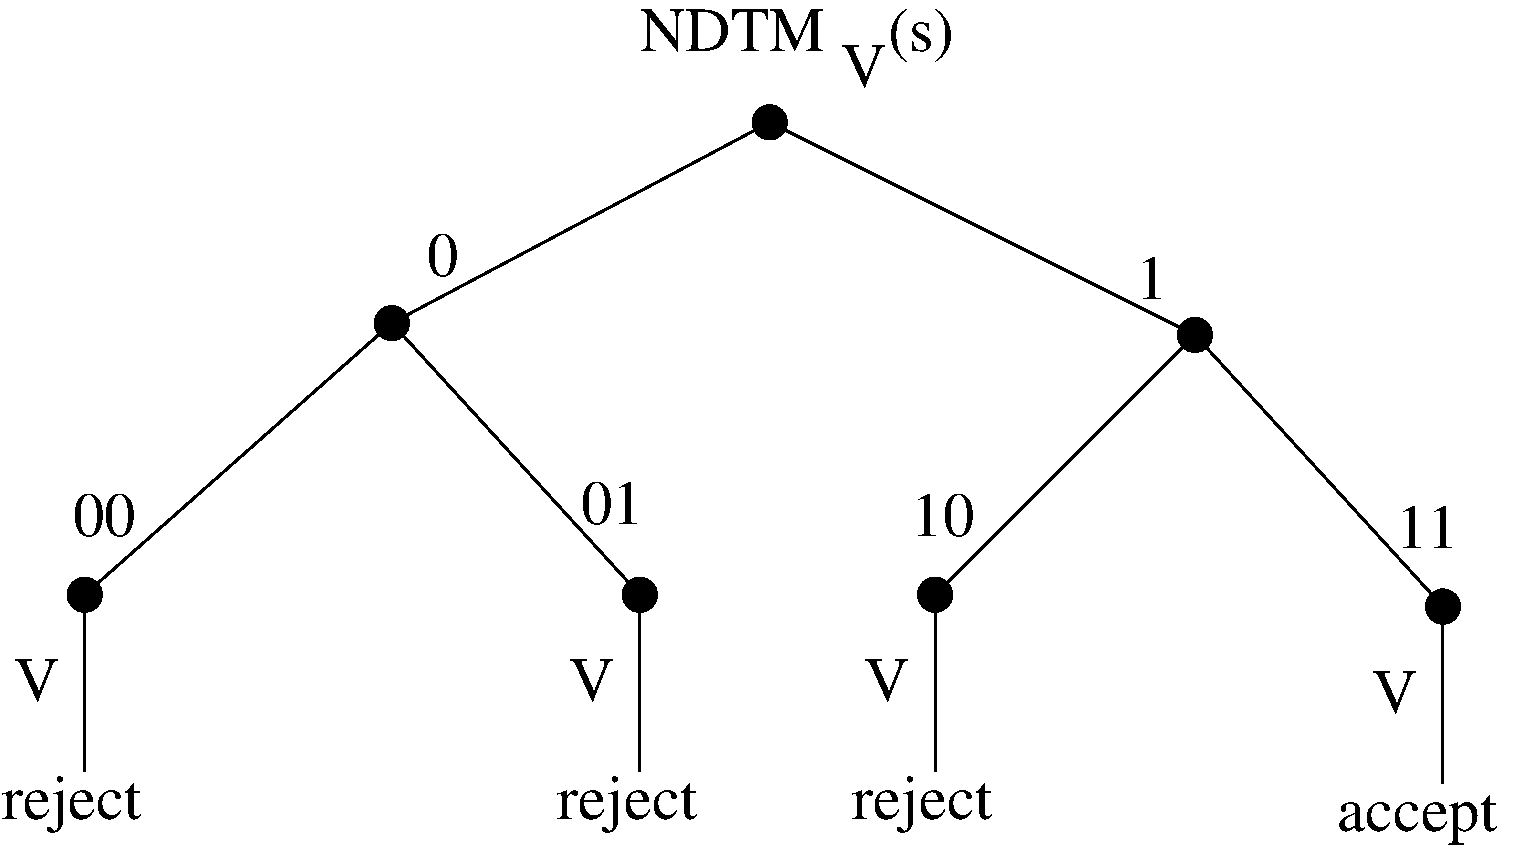
\includegraphics[height=0.2\textheight,keepaspectratio]{nondetverifier}
\caption{Generation of a certificate when the length is
known}\label{nondetverifier}
\end{center}
\end{figure}

Vice versa, we can transform this {\em NDTM$_V$} into a verifier: it
needs a certificate. Give as certificate a string representing the
choices needed for arriving at an accept state. Now simulate simulate
{\em NDTM$_V$} with those choices, of course with a deterministic TM
...

We have just (informally) shown that one can go back and forth between
a verifier+certificate (with known length) and a non-deterministic
Turing machine.



\subsection{Two definitions of \NP}

The class \NP can be defined in two way: the material in the previous
section contains the ingredients to prove their equivalence.

\grijs{
\begin{definitie} \NP with verifiers\\
\NP is the set of languages $L$ for which there exists a polynomial
verifier and a polynomial $p$ such that for each $s \in L$, there
exists a certificate $c$ vso that $|c| \leq p(|s|)$.  ~\\ ~\\
More formally: $L \in \NP$ if and only if

$~~~~~~~~\exists$ a polynomial TM $M$ and a polynomial $p: \N
\rightarrow \R^+$, so that

$~~~~~~~~~~~~~~~s \in L  \Leftrightarrow  \exists c \in \Sigma^{p(|s|)}$ met $M(\langle s,c \rangle) = accept$
\end{definitie}
}

The alternative definition of \NP uses non-deterministic Turing machines:
\grijs{
\begin{definitie} \NP with non-determinism\\
\NP is the set of languages accepted by a polynomial non-deterministic
Turing machine.
\end{definitie}
}

You should be able to argue that these two definitions define the same
set. Also, you must be able to argue that \NP is robust with respect
to the execution model.

Some examples of languages in \NP:

\begin{itemize}
\item 
since $\P \subseteq \NP$ (why?) each language in \P can serve as an example ...
\item 
pairs of isomorphic graphs (*)
\item 
graphs with a Hamiltonian cycle (*)
\item
non-connected graphs
\item
weighted graphs with between two given nodes a simple pad shorter than
a given number (*)
\item
Come up with something yourself!
\end{itemize}

Give for each example a description of a verifier and a certificate
for a string belonging to the language. Argue that it is
polynomial. Note that for the examples marked with (*), no polynomial
algorithm is known, neither whether one exists.

{\bf Careful:} \NP does means {\em non-deterministic polynomial},
and {\bf not} {\em non-polynomial}.

\subsection{Polynomial reduction}

In a previous chapter, we have reduced languages to each other: the
many-one reduction $\leq_m$ {\mbox is an example} (See
Page~\pageref{manyone}). The reduction below takes into account
complexity.

\grijs{\begin{definitie} Polynomial reduction\\
{ Given two languages $L_1\subseteq \Sigma_1^*$ (over alphabet $T_1$)
and $L_2\subseteq \Sigma_2^*$ (over $T_2$). We say that $L_1$
reduces polynomially to $L_2$ if there exists a mapping $f:\Sigma_1^*
\rightarrow \Sigma_2^*$ so that:
\begin{verse}
1. $\forall x\in \Sigma_1^*$: \ \ \ $x\in L_1\Leftrightarrow f(x)\in
L_2$\\[2mm] 2. There exists a deterministic TM that computes $f$ in
polynomial time.
\end{verse}
We denote this by $L_1 \leq_p  L_2$.}
\end{definitie}}


$\leq_p$ differs from $\leq_m$ only in the fact that the mapping must
be computable in poly-time. This makes $\leq_p$ finer than $\leq_m$:
if $A \leq_p B$ then $A \leq_m B$. Check whether some of the examples
of $\leq_m$ earlier in this course notes, were actually $\leq_p$?



\grijs{\begin{stelling} \label{transitief}
The relation $ \leq_p $ is transitive, or more explicitly:\\
if $L_1 \leq_p L_2$ and $L_2 \leq_p L_3$ then $L_1 \leq_p L_3$.
\end{stelling}}
\begin{proof}   
Let $f$ be the polynomial computable functions belonging to $L_1
\leq_p L_2$, and $g$ to $L_2 \leq_p L_3$; $M_f$ and $M_g$ are the
corresponding TMs: the first is a $T_f$-machine, the second a
$T_g$-machine, and $T_f$ and $T_g$ are polynomials. We prove that
%
the function $h = g\circ f$ is good for $L_1 \leq_p L_3$.

Clearly, $s \in L_1 \Leftrightarrow h(s) \in L_3$, and $h$ is
computable by a TM $M_h$: first let $M_f$ run on $s$, and when it is
finished, move the head to the left, and then let $M_g$. We just need
to show that $M_h$ is polynomial.

Let $s$ be a string with {\em a large enough} length be the input for
$M_h$. When $M_f$ is finished, the tape contains a string $s_f$ with
length at most $T_f(|s|)$. So, moving the head to the left costs at
most a polynomial (in $|s|$) amount of work. Executing $M_g$ on $s_f$
takes at most $T_g(T_f(|s|)$ time, so together we have as an upper
bound for the total time of $M_h$:
%
$T_f(|s|) + T_f(|s|) + (T_g \circ T_f)(|s|)$ which is polynomial in
$|s|$.
\end{proof}


The next theorem has the same feel as an earlier theorem about
$\leq_m$.

\grijs{\begin{stelling}\label{P_is_klein}
If $L_1  \leq_p  L_2$ and $L_2\in \P$ then $L_1 \in \P$.
\end{stelling}}

\begin{proof} Let $L_1\subseteq T_1^*$, $L_2\subseteq T_2^*$, and $L_1
\leq_p L_2$ via the function $f:T_1^*\rightarrow T_2^*$ that is
polynomial computable by TM $M_f$. Since $L_2\in \P$, there exists a
TM $M_2$ that decides $L_2$ in polynomial time. Construct TM $M$: it
executes $M_f$ and $M_2$ in sequence. Just as in the previous theorem,
we can prove that $M$ has polynomial time complexity. Moreover, $M$
decides $L_1$, so $L_1\in \P$.
\end{proof}

We name two languages equivalent if each can be polynomially reduced
to the other.


\grijs{\begin{definitie} Polynomial equivalence of languages\\
{
Two languages $L_1$ and $L_2$ are polynomial equivalent (denoted by
$L_1\sim_p L_2$) if 
\[ L_1 \leq_p  L_2 \mbox{ \ and \ } L_2  \leq_p  L_1\]
}\end{definitie}}



The wording in this definition is justified by 



\grijs{\begin{eig} The relation $\sim_p$ is an equivalence relation.
\end{eig}}
\begin{proof} We need to show that $\sim_p$ is reflexive, symmetric
and transitive. Reflexivity is trivial, symmetry follows directly from
the definition of $\sim_p$, and transitivity was already proven in
Theorem~\ref{transitief}.
\end{proof}

As with any equivalence relation, we van consider the equivalence
classes induced by the relation. They form a partition. \P is consists
of exactly three equivalence classes. Make sure you understand this.


\subsection{NP--complete}

Within $\NP$, there exists a special class of languages: de most
difficult of all in \NP !

\grijs{
\begin{definitie}\label{defnpc} The class $\NP$--complete\\
A language $L$ is $\NP$--complete if and only if 
\begin{verse}
1. $L\in \NP$ and \\[2mm]
2. for each language $L'\in\NP$, it is true that $L' \leq_p  L$.
\end{verse}
We denote the class of $\NP$--complete languages by $\NPC$.
\end{definitie}
}


Informally, an $\NP$--complete language is so difficult that any other
language can be translated to it in polynomial. In terms of problems:
a problem is $\NP$--complete if it has an solution (in the form of an
algorithm) so that every other $\NP$ problem has a solution that can
be deduced from the $\NP$--complete solution by a polynomial reduction
van de $\NP$--complete. A priori, it is not clear whether
$\NP$--complete languages exist at all, neither whether $\NPC$
coincides with $\NP$ or $\P$. However, the relevance of this class is
captured in the following theorem:

\grijs{\begin{stelling}$ $
\begin{verse}
1. \NPC is an equivalence class for $\sim_p$.\\[2mm]
2. If $\NPC\cap\P\neq \emptyset$ then $\NP=\P$.
\end{verse}
\end{stelling}}
\begin{proof} ~~
\begin{verse}
1. Suppose $L_1,L_2\in\NPC$. By the definition of $\NP$--completeness,
both $L_1 \leq_p L_2$ and $L_2 \leq_p L_1$. So,$L_1$ and $L_2$ are
polynomial equivalent. The class $\NPC$ is therefore part of one
equivalence class $C$. Moreover, suppose that $L' \in C\setminus \NPC$,
then for every $L\in\NP$, $L \leq_p L'$, meaning $L' \in \NPC$, so $C = \NPC$.


2. Suppose $L\in\P \cap\NPC$. Consider any other language $L'\in
\NP$. Since $L\in\NPC$, we know that $L' \leq_p L$. Since also
$L\in\P$, it follows from Theorem~\ref{P_is_klein} that $L'\in
\P$. So, $\NP=\P$.
\end{verse}
\end{proof}

The previous previous theorem shows that if one $\NP$--complete
problem can be solved in polynomial time, all problem in \NP can be
solved in polynomial time. There is however lots of evidence that \NP
does not equal $\P$.\footnote{On the other hand ... Donald Knuth
believes in $\P = \NP$.}

Figure~\ref{NP-venn} shows the two possibilities: either $\P \neq \NP$
or $\P = \NP$.

\begin{figure}[ht]
\begin{center}
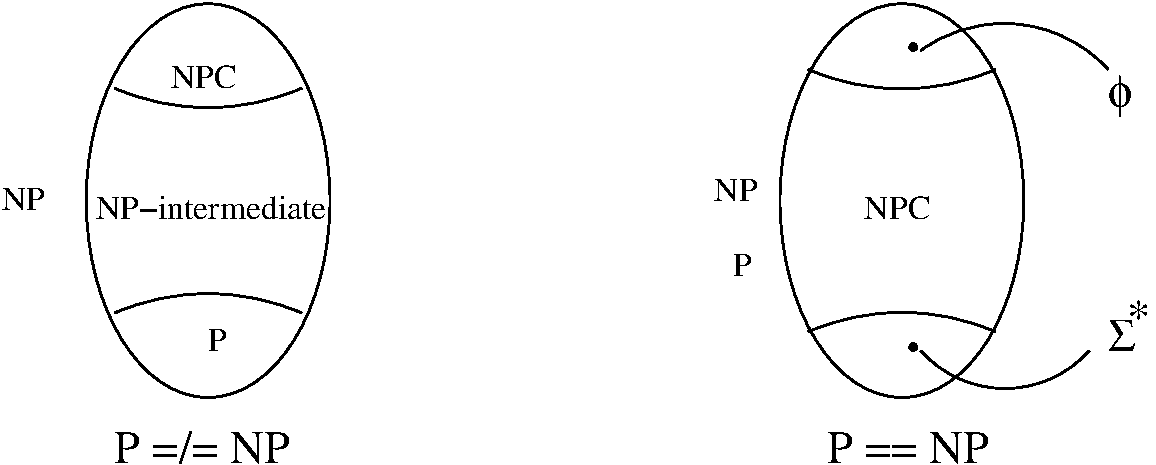
\includegraphics[width=0.7\linewidth,keepaspectratio]{NP-venn}
\end{center}
\caption{The possible relation between $\P$, $\NP$ and $\NPC$
 \label{NP-venn}}
\end{figure}
The set $\NP$-intermediate is not empty if $\P \neq \NP$. A candidate
$\NP$-intermediate problem is {\em graph isomorphism}.

The first problem proven to be in \NPC is the {\bf satisfiability}
problem, often abbreviated by SAT. We need some definitions to specify
the SAT language. Let $U = \{u_1,u_2,\ldots,u_n\}$ a finite set of
boolean variables, i.e. each variable $u_i$ can take the values {\em
true} or {\em false}.  A literal (or atom) from $U$ we mean either one
of the variables $u_i$, or its negation denoted by $\neg {u}_i$ (read
this as {\em not $u_i$}). Consider a formula in Conjunctive Normal
Form (CNF) over $U$, i.e. a conjunction of disjunctions of literals
over $U$ as in the following example:
%
$C= (u_1 \vee u_2) \wedge (u_2 \vee \neg u_4 \vee u_7) \wedge  (\neg u_2 \vee u_3)$.

The SAT problem is: given a formula in DNF, does there exist a truth
assignment to the variables so that the formula is true?

More precisely, SAT is the language of DNF formulas that have a
satisfying assignment.

Stephen A. Cook\footnote{Turing award 1982} proved in 1971



\grijs{\begin{stelling} The Cook-Levin Theorem.
$SAT \in \NPC$
\end{stelling}}

We do not study the proof of this theorem in this course. What you
should be able to do is: show that $SAT \in \NP$, once using the
non-deterministic definition of \NP, and once using the verifier
definition. What is the size of the certificate? How did you encode
the language?

Once the first $\NP$--complete problem was know, many more
$\NP$--complete were found. Here are just a few examples: Hamiltonian
graphs, N-colorable graphs, subgraph isomorphism, the knapsack
problem, pancake sorting, 0-1 integer programming, lots of
combinatorial problems and even puzzles like Sudoku.

A language $L$ that fulfills only the second condition of Definition
\ref{defnpc}, is named {\em NP-hard}. One also uses $\NP$--hard for
optimization problems whose decision version is $\NP$--complete. There
exist $\NP$--hard problems that are not $\NP$--complete (i.e. they
are not in \NP): $SAT$ even has a polynomial reduction to $H_{TM}$,
and so has every $\NP$. Work this one out!


\subsection{Examples of polynomial reductions}

\subsubsection{SAT to 3-SAT}

3-SAT is SAT with the restriction that each disjunction in the DNF has
exactly three literals. One formula in 3-SAT is
%
$(a \vee b \vee \neg c) \wedge (\neg a \vee b \vee c)$. Every formula
in DNF can be transformed to that format. Consider each disjunction in
the formula. There are three cases:
\begin{itemize}
\item 
the disjunction contains less than three literals: repeat one of the
literals until there are three
\item 
the disjunction contains exactly three literals: just leave them
unchanged
\item 
the disjunction contains strictly more than three literals: the
disjunction is of the form
%
$a_1 \vee a_2 \vee  ... \vee a_n$ met $n > 3$.

Take a new boolean variable, say $b$, and replace this one disjunction
by the two disjunctions
\begin{verse}
(1) $b \vee a_{n-1} \vee a_n$ and

(2) $\neg b \vee a_1 \vee a_2 \vee  ... \vee a_{n-2}$
\end{verse}

Repeat all this until no disjunction contains more than three literals.
\end{itemize}

Now check the following about the transformation:
\begin{verse}
* a formula $\in SAT$ is mapped to a $ \in$ 3-SAT

* a string $\notin SAT$ is mapped to a string $ \notin$ 3-SAT

* the transformation can be implemented on a polynomial TM
\end{verse}



3-SAT $\in \NP$: members of 3-SAT have a polynomial certificate and a
verifier that uses it. Putting things together: 3-SAT $\in \NPC$. You
should now be able to show that n-SAT $\in \NPC$ whenever $n \geq 3$,
but ...

\paragraph{2-SAT} has a polynomial\footnote{in the number of occurring
literals} algorithm. One find in literature even that 2-SAT has a
linear algorithm, but that is on a random access machine, not on a
TM. In any case, 2-$SAT \notin \NPC$ ... or is it?


\subsubsection{reducing 3-SAT to $k$-CLIQUE}

The language $k$-CLIQUE consists of tuples $\langle G,i \rangle$
in which $G$ is a graph with a clique of size $i$, or otherwise said:
$G$ contains a subgraph isomorphic to $K_i$. Two examples show how the
reduction works:

\begin{vb}
The formula in 3-SAT is
$(a \vee b \vee c) \wedge (a \vee \neg b \vee \neg c) \wedge (\neg a \vee b \vee \neg c) \wedge (\neg a \vee \neg b \vee c)$

\begin{figure}[h]
\begin{center}
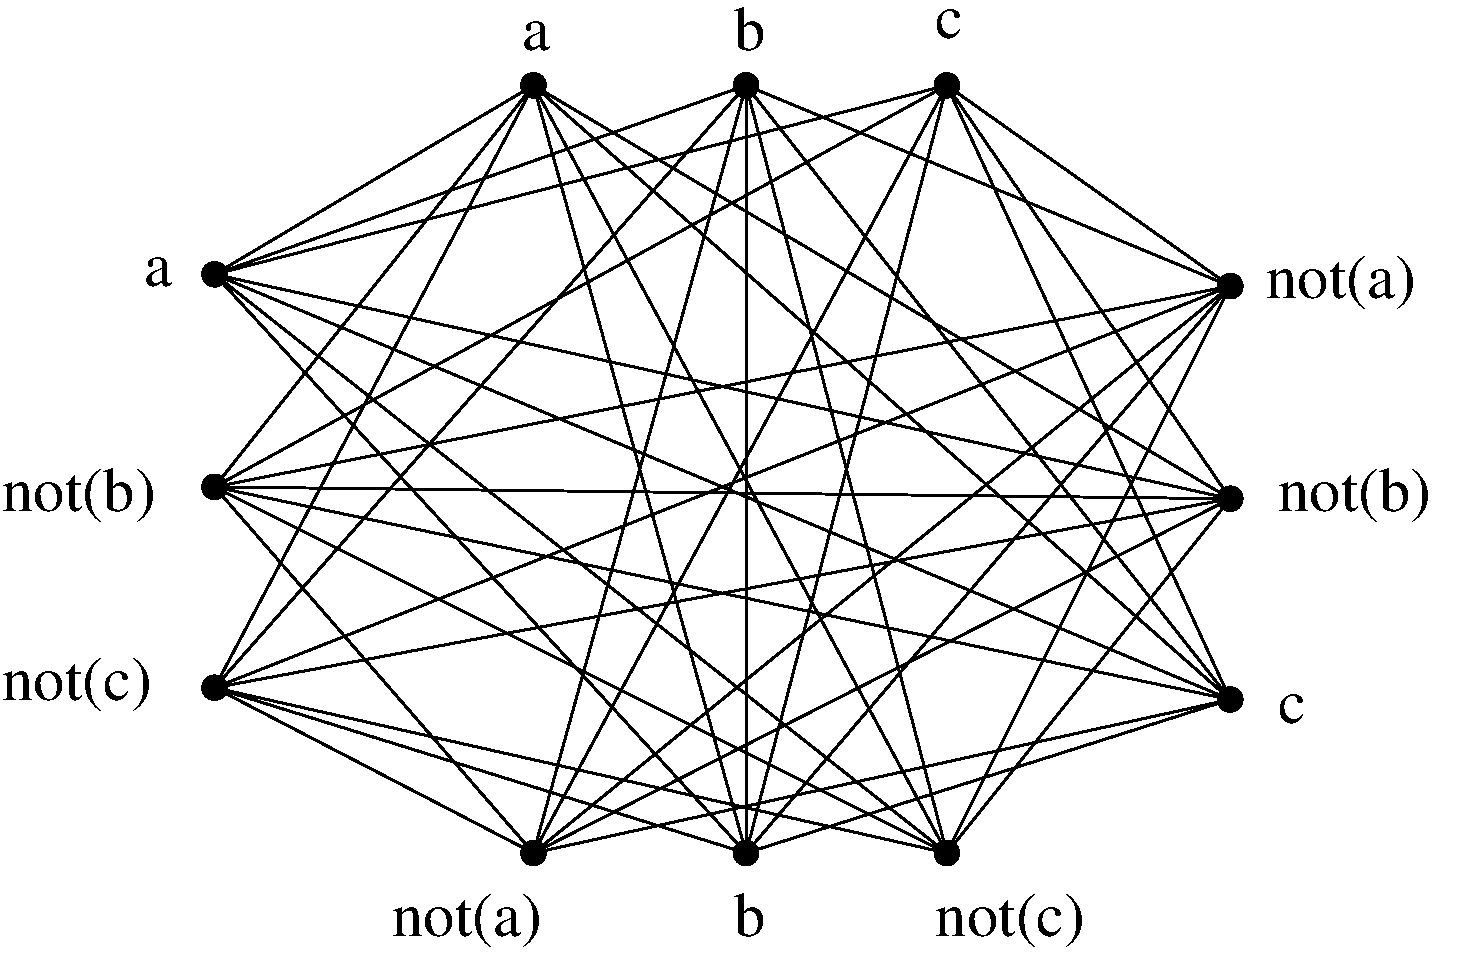
\includegraphics[height=0.2\textheight,keepaspectratio]{satclique}
~~~~~~~~~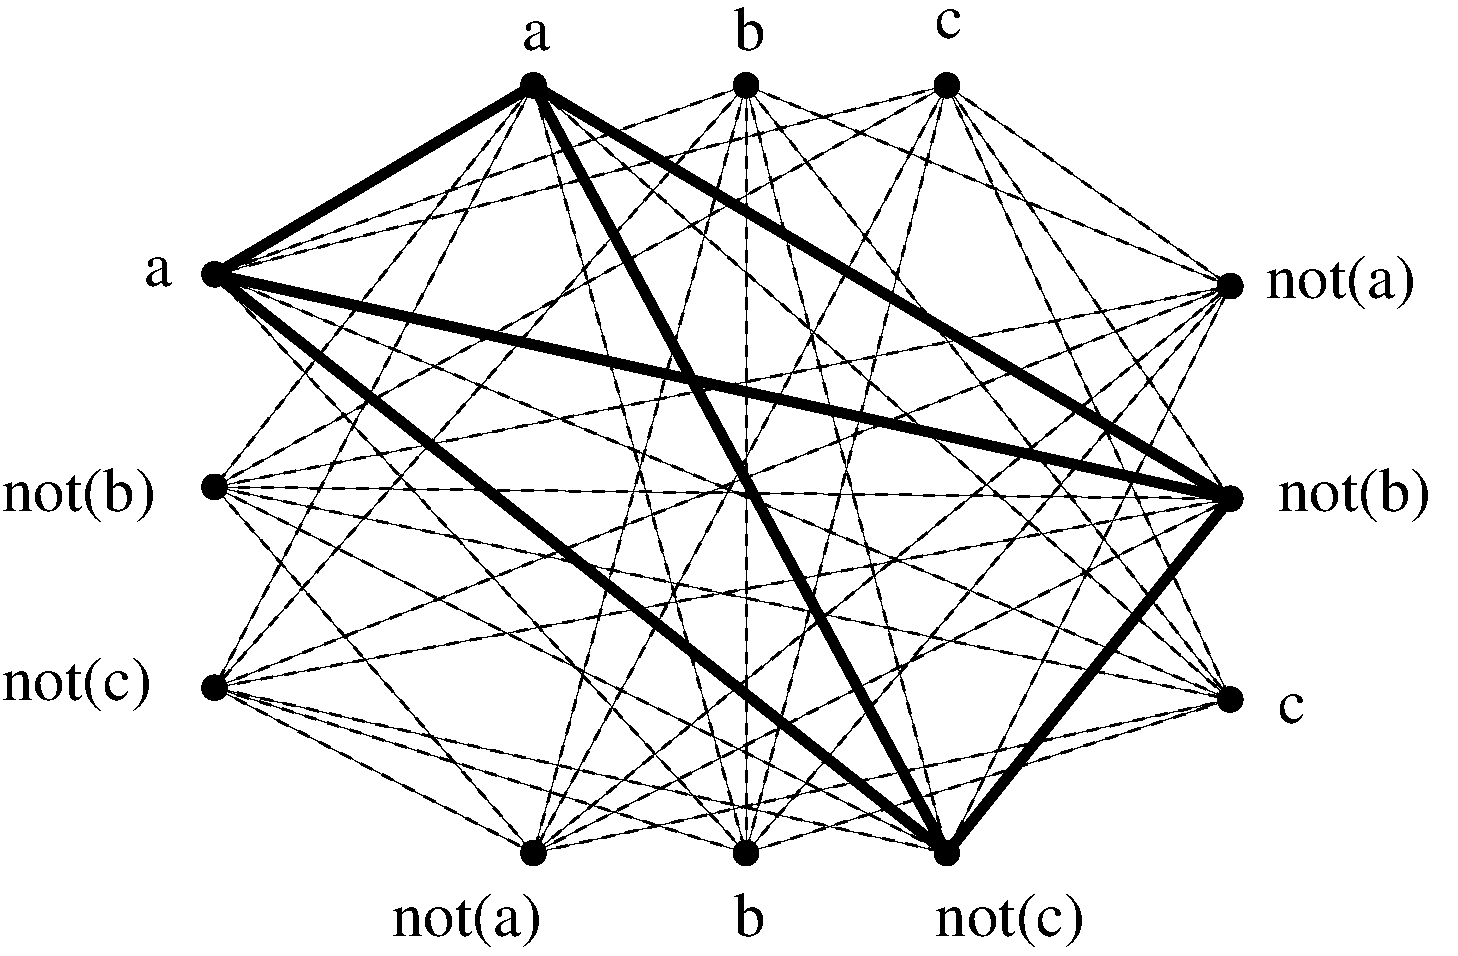
\includegraphics[height=0.2\textheight,keepaspectratio]{satcliquesol}
\caption{The graph corresponding to the first formula, and a 
4-clique}\label{satclique}
\end{center}
\end{figure}

Figure~\ref{satclique} shows at the left the graph resulting from the
reduction:
\begin{verse}
- each occurrence of a literal corresponds to one vertex with as its
name the literal

- there is an edge between two vertices that are {\em compatible}: $p$
and $\neg p$ are not compatible and two vertices from the same
disjunction are not compatible either
\end{verse}

The incidence matrix of this graph can be computed in polynomial
time. The required clique size (4 in the example) is the number of
disjunctions in the formula.
\end{vb}

Convince yourself that the graph has a clique of the required size if
and only of the formula belongs to SAT.


\begin{vb}
The reduction can be applied to smaller disjunctions as well. We take
as formula: $(a \vee b) \wedge (\neg a \vee b) \wedge (a \vee \neg b)
\wedge (\neg a \vee \neg b)$


\begin{figure}[h]
\begin{center}
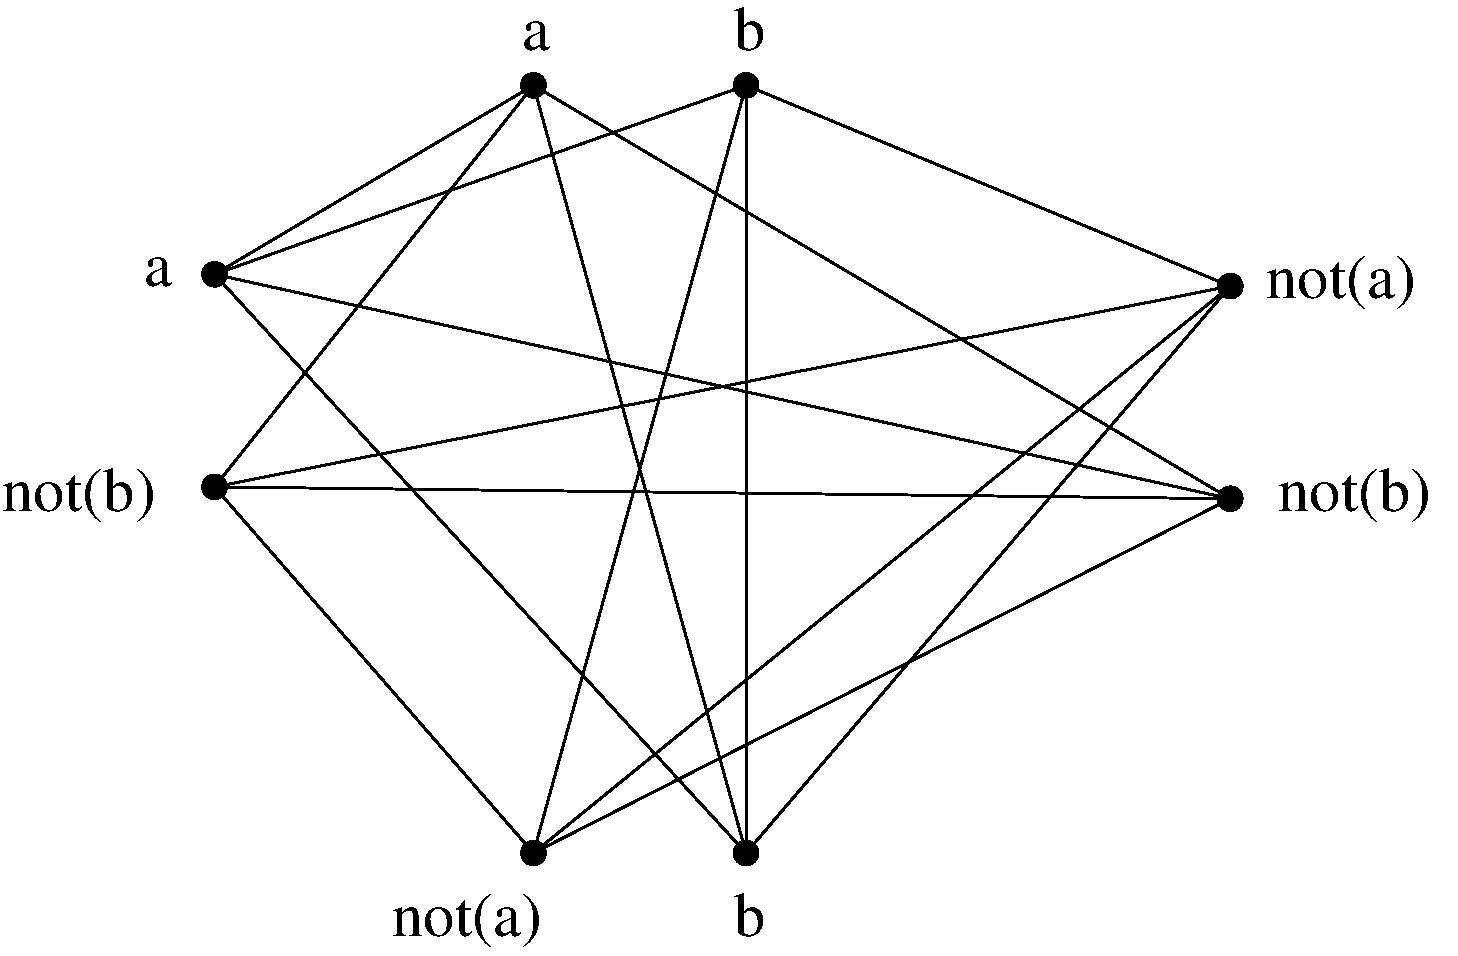
\includegraphics[height=0.2\textheight,keepaspectratio]{satclique2}
\caption{The graph corresponding to the second formula: there is no
4-clique}\label{satclique2}
\end{center}
\end{figure}

Because the graph has no 4-clique, the formula does not belong to
SAT. Of course, the graph does have k-cliques: the maximal k gives us
the maximal number of disjunctions that can be true at the same
time. In this way, two optimization problems are connected by a
polynomial reduction.

\end{vb}

% \newpage
{\bf Selfie:} 
\begin{verse}
- did you see a correspondence between the reduction from SAT to 3-SAT
and how we put a CFG into Chomsky Normal Form?

- reduce $3$-SAT to SAT

- which was easy because $3$-SAT $\subsetneq SAT$, so here are some
general questions:

\begin{verse}
* does $A \subseteq B$ and $A \in \P$ imply that $B \in \P$?

* does $A \subseteq B$ and $A \in \NP$ imply that $B \in \NP$?

* does $A \subseteq B$ and $A \in \NPC$ imply that $B \in \NPC$?

* does $A \subseteq B$ and $B \in \P$ imply that $A \in \P$?

* does $A \subseteq B$ and $B \in \NP$ imply that $A \in \NP$?

* does $A \subseteq B$ and $B \in \NPC$ imply that $A \in \NPC$?

\end{verse}
\end{verse}


\subsection{Why are some problems to difficult?}

For SAT, one could argue as follows: there are $2^n$ possible
assignments ($n$ is the number of boolean variables), and our
intuition tells us that we need to check all of them to find the good
one (or on average half of them) ...

For Hamiltonian cycles, we would argue: the number of simple cycles in
a graph is exponential in the number of vertices, and our intuition
tells us ...


For Minimal Spanning Tree, we would argue: the number of spanning
trees for a graph with $n$ vertices can be at worst $n^{n-2}$ - that
is even worse than exponential, so our intuition ... would be totally
wrong. Indeed, we saw a greedy polynomial algorithm for this
problem: Prim and Kruskal. For MST, we relied on a graph theorem and
that guaranteed the correctness of a polynomial algorithm without the
need to check all possibilities.

Perhaps we have not yet proven the the right theorem for SAT, the
theorem that results in a polynomial algorithm for SAT, but if we do,
we will need to adjust our intuition just as with Karatsuba and
multiplication.

\section{The time hierarchy}\label{timeshierarchie}

As far as we discussed it, the structure of \P is rather uniform.
The time hierarchy theorem changes that: below is a correct version,
but not the strongest possible one:

\grijs{
\begin{stelling} 
$DTIME(f) \subsetneq DTIME(f^2)$ for every {\em time-constructible}
$f$.
\end{stelling}
}

Loosely speaking, a function $f$ is time-constructible if $f$ can be
computed on a TM in $O(f)$ steps and $f(n) \geq n$. Most probably, you
will never during your life meet a (non-trivial)
non-time-constructible function :-)

R. Stearns and J. Hartmanis proved in 1965 the first version of the
time hierarchy theorem, quite a few years before the notion of
$\NP$--completeness came to life. For that - and other things - they
got the Turing award in 1993.

It is important to realize that strictly more problems can be solved
with a $O(n^4)$ algorithm than with $O(n^2)$: time is a resource, and
it is limited. This is a good moment to think about the following:
\begin{verse}
- how many languages are in $DTIME(n^k)$?

- how many languages are in \P?

- how many languages are in \NP?

- if you answered {\em countable infinite} to one or more of these
questions, would that also be effectively enumerable?
\end{verse}


\section{co-\NP}

Since the definition of \NP treats elements of the language
differently from the one not in the language, it is worthwhile
investigating the complement of languages in \NP:

\grijs{
\begin{definitie} co-\NP: 
co-\NP = $\{L | \overline{L} \in \NP\}$
\end{definitie}
}

Be careful: co-\NP does not equal $\overline{\NP}$. The latter
contains non-decidable languages like $A_{TM}$, but every language in
co-\NP is decidable (why?). Some examples provide the intuition that
co-\NP might be different from \NP.

\begin{verse}
- $SAT \in \NP$ because we have a short (polynomial) certificate for
satisfiable formulas; $\overline{SAT} \in co$-$\NP$; how about
certificates for elements in $\overline{SAT}$; $\overline{SAT}$
contains the formulas for which no assignment is satisfying ... could
that have a short certificate? nobody knows

- consider $TAUTOLOGY$; it is the language of formulas that are true
for {\bf every} assignment to the variables; $\overline{TAUTOLOGY}$
is definitely in $\NP$: a short certificate would be an assignment
that makes the formula false; but a short certificate that can be
verified in polynomial time so in case the formula is a tautology
... nobody knows

- the set of sorted sequences is a language in $\NP$; a certificate
for a non-sorted sequence would be an index $i$ so that the i$^{th}$
element is larger than the (i+1)$^{th}$ element; so the set of sorted
sequences belongs to co-$\NP$ as well; yu could have argued: the set
of sorted sequences is in \P, so also in co-$\NP$; that is right, but
you would have missed thinking up a non-trivial polynomial certificate


- COMPOSITE (the set of composite numbers) has a short certificate: a
divisor of the number; it is difficult to think of a short
certificate for PRIME (which is $\overline{COMPOSITE}$; on the other
hand, since 2004 we know that PRIME $\in \P$, so this short
certificate indeed exists ... (can you think of one?)
\end{verse}


After these examples, you should understand that $\P \subseteq \NP
~\cap$ co-\NP, and that $\NP = $co-\NP is not a trivial question. You
must also be able to argue that $\P = \NP$ implies $\NP = $ co-\NP.
And what if $SAT \in$ co-$\NP$?

\section{$\NP$--complete or $\P$?}

In this section, we merely want to point out that the details how a
problem is specified really matter. Consider the following two
languages:

\begin{verse}
- $k$-CLIQUE = $\{\langle G,i \rangle|$ i an integer, G a graph with an i-clique$\}$

- 7-CLIQUE = $\{\langle G \rangle|$ G a graph with an 7-clique$\}$
\end{verse}

We showed that $k$-CLIQUE is in \NPC (we reduced SAT to it), but
7-CLIQUE is polynomial: let $n$ be the number of vertices in G; there
are $C_n^7$ subsets of vertices that potentially form a
7-clique. Checking one of them is polynomial in the size of G, say
$O(n^c)$ for some $c$. Moreover, $C_k^7 = O(n^7)$ so we have a naive
algorithm with time complexity $O(n^{c+7})$. The encoding of G has
size $O(n^2)$, so the 7-CLIQUE is in \P.

This phenomenon shows up quite often: by keeping one or more
parameters of the problem constant, we get a polynomial version of an
\NP-complete problem.

Reconsider the following two problems:

\begin{verse}
- $A_{TM} = \{\langle M,w \rangle| w \in L_M\}$

- $E_{TM} = \{\langle M \rangle| \epsilon \in L_M\}$
\end{verse}

By keeping one parameter in $A_{TM}$ fixed, we get $E_{TM}$. Did that
pay off in this case?



\section{Space complexity}

Space is a resource: has your Java program ever stopped unexpectedly
because of stack overflow? Or has the progress of your program ever
become unacceptably slow because of excessive swapping or garbage
collection? If so, you know that space is a (limited) resource, and
space complexity deals with it. One could try to define the space
complexity of an algorithm (on a TM) as the number of cells that are
read/written on the tape. That would not be so useful:
\begin{verse}
- for non-trivial problems, the input needs to be read completely, so
space complexity could not be sublinear: the space cost of the input
is indeed unavoidable

- on the other hand, many algorithms need very little extra {\bf
extra} space (besides the input)
\end{verse}

The latter should be familiar. E.g. testing whether a sequence is
sorted needs an index and a fixed amount of space for comparing the
two consecutive cells in the sequence: a constant space overhead.

Before we start with the definitions, think about this: one can reuse
space, one cannot reuse time! So one expects to need {\em less} space
than time for solving a given problem.

The definition of space complexity is based on a Turing machine model
with
\begin{verse}
- one read-only tape containing the input string

- one read-write tape
\end{verse}
The space cost of an algorithm is equal to the number of cells used on
the R/W tape.

\grijs{
\begin{definitie}
DSPACE(f) is the set of languages decided by a deterministic Turing
machine using $O(f)$ cells on the R/W-tape.
\end{definitie}
}

\grijs{\begin{eig} \label{grootte_van_string}
If the function $f$ is computed on a $T$-time TM, then
%
$|f(s)| \leq T(|s|)$.
\end{eig}}
This essentially says that a TM cannot write on more tape cells than
it makes steps.

Now, you argue that $DTIME(f) \subseteq DSPACE(f)$. 


\grijs{
\begin{definitie}
$\PSPACE = \cup_{k\geq 1} DSPACE(n^k)$
\end{definitie}
}

It should be clear now that $\P \subseteq \PSPACE$.

Just as for time, there exists a space hierarchy
theorem. A.o. $DSPACE(f) \subsetneq DSPACE(f^2)$ for {\em decent} $f$.

\grijs{
\begin{definitie}
$\NPSPACE$ is like \PSPACE, but with non-deterministic Turing
  machines.
\end{definitie}
}

The inclusion $\PSPACE \subseteq \NPSPACE$ is easy to prove, and one
might suspect that $\PSPACE \neq \NPSPACE$, or that it is unknown.
Surprise ... $\PSPACE = \NPSPACE =$ co-$\PSPACE$. The fact that
non-determinism does not change $\PSPACE$ is related to the fact that
space can be reused: a non-deterministic TM can be simulated
deterministically with little space overhead. That provides the
intuition that co-$\NPSPACE$ must equal $\NPSPACE$.


\paragraph{Less than linear space?} This is also possible. Consider the
language of even numbers: one can decide it with no extra space at all!
This works actually for all regular languages. There exist also
languages beyond RegLan that can be decided in sublinear space. As an
example, we consider the problem to decide whether there exists a path
between two given vertices in a given directed graph $(V,E)$. We
describe (in pseudo-code) a $log(n)^2$-space algorithm: $n$ is the
number of vertices.

\newpage
\begin{algorithmic}
\Function {existspath}{a,z,l}
\If {$(l = 0)$}
\State{return(a = z)}
\EndIf
\If {$(a,z) \in E$}
\State{return(TRUE)}
\EndIf


\ForAll {$(v \in V$}
   \If {{\sc existspath}$(a,v,l/2)~ \wedge~ ${\sc existspath}$(v,b,l-l/2)$}
   \State{return(TRUE)}
   \EndIf
\EndFor
\State{return(FALSE)}
\EndFunction
\end{algorithmic}

{\sc existspath}$(a,z,n)$ returns TRUE if there exists a path from a
to z with length at more l. Its time complexity is horrible. If you
imagine it is executed on a classical machine (your laptop), you see
that no more than $\log(n)$ stack frames are needed, and that each
stack frame has size at most $\log(n)$ bits. The algorithm can be
implemented on a DTM with the same space complexity.

It is also interesting that one can trade space for time: you can make
a version of \mbox{{\sc existspath}} that uses less time, but more
space, e.g. by using a depth-first backtracking search through the
graph, while you remember the visited nodes: that is $O(n)$.

Algorithms (and problems requiring them) that use log-space are
interesting enough to warrant their own class:

\grijs{
\begin{definitie}
$\LL = DSPACE(\log)$
\end{definitie}
}


Log-space algorithms are important, e.g. in the context of large
databases, or long DNA-sequences: with the log of the space taken by a
database, you can keep a fixed number of pointers (in binary) and
often that is often enough to traverse the database and answer a
set of queries.

\newpage
\section{A sequence of inclusions}

We know and understand enough at this point to justify the following
sequence of inclusions:

\begin{verse}
$\LL \subseteq \NL \subseteq \P \subseteq \NP \subseteq \PSPACE
  = \NPSPACE \subseteq \EXP$
\end{verse}

Thanks to the hierarchy theorems, we know for sure that 
$\LL \neq \PSPACE$ and $\P \neq \EXP$. This means that some of the
inclusions are strict, but currently nobody knows which ones.


\section{Complexity and Chomsky hierarchy}

What is the connection between the complexity of a language and its
place in the Chomsky hierarchy?

It is easy to see that a regular language can be decided in $O(n)$
steps if $n = |s|$ on an FSA. Whether this is also possible on a DTM
remains to be proven ... by you. One needs very little extra space to
decide a regular language, actually none at all. Besides, only regular
languages can be decided with strictly less than $\log$-SPACE.

Context free languages can be recognized by a general $O(n^3)$
algorithm (on a 3-tape TM) algorithm known by the names of the authors
as Cocke-Younger-Kasami. It is a form of {\em chart} or {\em tabular
  parsing}, or dynamic programming. Moreover, you only need linear space on the stack of the PDA, so $CFL \subset SPACE(n)$.

The class of non-deterministic LBA decides languages by using no more
than the space occupied by the input, so context-sensitive languages
constitute the class {\bf NSPACE}(n).


% \newpage
\section{Conclusion}

A basic concern in the study of algorithm complexity \footnote{Its
  roots are at least 150 years old.} is the characterization of {\em
  fast} algorithms in a formal way, and also of problems allowing a
fast algorithm. Very soon it was realized that the size of the input
to the algorithm has an important role in this characterization.

Only in 1965 did Jack Edmonds propose to define {\em fast} as {\em
  polynomial in the input length}: this followed the general feeling
that a polynomial algorithm might be fast enough, but an exponential
one certainly is not. The (decision) problems with a fast solution
form together the class $\P$. Problems not in $\P$ are considered {\em
  intractable} - at least for practical means.

By the end of the 1960's, it became clear that for some seemingly
simple problems (like SAT) nobody was able to construct a polynomial
algorithm. Steve Cook cooked up the notion of {\em verifiable in
  polynomial time} and the class $\NP$ was born. In 1971 Cook proved
that within $\NP$ there exists a class of {\em most difficult}
problems, i.e. the class $\NP$-complete, and that $\NP$-complete is
not empty. Leonid Levin (USSR) proved the same result almost
simultaneously and independently: he published in Russian, and - also
because of the cold war - his result was not well-known in the West.
The finishing touch was the understanding that one problem in
$\NP$-complete $\cap \P$ is enough to collapse $\P$ and $\NP$, or to
put it in words: verifying [a solution] would be as difficult as
computing [it] (module the exponent in the polynomial of
course). However, the strict inclusion of $\P$ in $\NP$ is an open
problem. It feels like betting on the opposite is a bad choice,
because there are so many NP-complete problems for which researchers
have tried to find a polynomial algorithm ... and they failed. Still,
you should make up your own mind about this fundamental problem in CS!

Currently, the separation between $\NP$-complete and $\P$ is important
because one should not hope for an efficient solver for intractable
problem (for ever growing input size). Most everyday real problems
are $\NP$-complete (vehicle routing, exam rostering ...) or they have
algorithms with an impractical exponent (PRIME). Fortunately,
efficient solvers based on different principles have been developed,
as well as the theory on which they are based. We have very fast
probabilistic algorithms for checking whether a number is prime (they
fail almost never), we have heuristics and approximation schemes for
optimization problems for which we have no polynomial algorithm (at
this moment). Sometimes we can fix a parameter and that results in a
tractable problem. Complexity theory has ramifications in other
scientific activities like cryptography, quantum computing, information
theory, circuit-design ... , but for now, the central question
is $\P =? \NP$.

% \newpage
\section{References}
\begin{itemize}
% \item S.A. Wiitala, ``Discrete Mathematics, a unified approach'',
% McGraw--Hill Book Company, 1987
% \item A.K. Dewdney, ``The Turing Omnibus, 61 Excursions in computer
% science'', Computer Science Press, 1989
% \item J.K. Truss, ``Discrete Mathematics for Computer Scientists'', 2nd edition, 
% Addison--Wesley, 1999
\item Sanjeev Arora and Boaz Barak, ``Computational Complexity: A Modern Approach'',
Cambridge University Press
\end{itemize}



